\section{Desarrollo: Caso 3, configuración VFA-CFA con red cero-polo}
\label{sec:desarrollo_c3}

\subsection{Diseño}
\label{sec:diseno_c3}

Al compuesto del Caso 2 se le agrega una red cero-polo a la salida del VFA (\autoref{eq:red_RC}, \autoref{sec:adelanto}): $C_x$ en paralelo con $R_x$ en serie entre la salida del LM324 y la entrada del CFA, y $R_y$ a tierra. Es la compensación con red a la salida del amplificador básico, donde el cero se ubica sobre el segundo polo del VFA ($D_x = z_x/p_2 \cong 1$, apunte Ec.~6.50 y 6.51) para cancelarlo, y el polo de la red queda una octava por encima, $f_{px} = 2f_{zx}$.

Con $\omega_{px}/\omega_{zx} = 1 + R_x/R_y = 2$ resulta $R_x = R_y$; adoptando $R_y = \SI{1}{k\ohm}$ queda $R_x = \SI{1}{k\ohm}$ y, para $f_{zx} = f_2$, $C_x = 1/(2\pi R_xf_2) = \SI{31,45}{pF}$. La atenuación de la red es $A_c(0) = R_y/(R_x+R_y) = 0{,}5$, por lo que se duplica la ganancia del CFA, $G_0' = G_0/A_c(0) = 40$, para conservar $T_0$ y $f_g$; entonces $R_1' = R_2/(G_0'-1) = \SI{21,03}{\ohm}$. El aumento de ganancia eleva $R_{eff}' = R_2 + r_iG_0' = \SI{1620}{\ohm}$ y baja el polo del CFA a $\SI{20,5}{MHz}$ (10 veces $f_g$); el CFA aislado conserva un margen de fase de $\ang{76,4}$.

\begin{table}[H]
\centering
\caption{Diseño VFA-CFA con red cero-polo: expresiones, cálculo y valores.}
\label{tab:parametros_vfa_cfa_red}
\footnotesize
\setlength{\tabcolsep}{4pt}
\begin{tabular}{>{\raggedright\arraybackslash}p{0.31\textwidth} >{\centering\arraybackslash}p{0.2\textwidth} >{\centering\arraybackslash}p{0.27\textwidth} >{\centering\arraybackslash}p{0.13\textwidth}}
\toprule
\textbf{Parámetro} & \textbf{Expresión} & \textbf{Cálculo} & \textbf{Valor} \\
\midrule
Ganancia global, $K$, $R_i$, $R_f$ & -- & igual que Caso 2 & \autoref{tab:parametros_vfa_cfa} \\
Resistencia a tierra de la red $R_y$ & elegida & -- & \SI{1}{k\ohm} \\
Resistencia serie de la red $R_x$ & $R_y(\omega_{px}/\omega_{zx}-1)$ & $1\text{ k}\Omega\cdot(2-1)$ & \SI{1}{k\ohm} \\
Capacitor de la red $C_x$ & $1/(2\pi R_xf_{zx})$ & $1/(2\pi\cdot 1\text{ k}\Omega\cdot 5{,}06\text{ MHz})$ & \SI{31,45}{pF} \\
Cero de la red $f_{zx}$ & $f_2$ & -- & \SI{5,06}{MHz} \\
Polo de la red $f_{px}$ & $1/(2\pi C_x(R_x\parallel R_y))$ & $2f_{zx}$ & \SI{10,12}{MHz} \\
Atenuación de la red $A_c(0)$ & $R_y/(R_x+R_y)$ & $1/2$ & \num{0,5} \\
Ganancia del CFA retocada $G_0'$ & $G_0/A_c(0)$ & $20/0{,}5$ & \SI{40}{V/V} \\
Resistencia local a tierra $R_1'$ & $R_2/(G_0'-1)$ & $820/39$ & \SI{21,03}{\ohm} \\
Resistencia efectiva $R_{eff}'$ & $R_2+r_iG_0'$ & $820+20\cdot 40$ & \SI{1620}{\ohm} \\
Ganancia de lazo en continua $T_0$ & $K\,A_{d0}\,A_c(0)\,G_0'$ & $0{,}1\cdot10^5\cdot0{,}5\cdot40$ & \num{200000} (\SI{106}{dB}) \\
Separación de polos $D_p$ & $f_{px}/f_1$ & $10{,}12\text{ MHz}/10\text{ Hz}$ & \num{1012000} \\
\bottomrule
\end{tabular}
\end{table}

\subsection{Resultados analíticos}
\label{sec:analitico_c3}

Con el cero cancelando el segundo polo del VFA, el producto $A_1A_c$ queda con los polos $f_1$ y $f_{px}$, y la ganancia de lazo es $T(s) \cong T_0/[(1+s/\omega_1)(1+s/\omega_{px})]$ con el mismo $T_0$ y $f_g$ que en el Caso 2. Como $D_p$ se duplicó, $Q_p^2 = f_g/f_{px} = 0{,}198$ es la mitad que en el Caso 2 y los polos de lazo cerrado resultan reales y distintos (respuesta sobreamortiguada, $\zeta>1$). La \autoref{tab:analitica_c3} reúne los resultados; el margen de fase del modelo simple se verificó también con la fórmula del apunte.

\begin{table}[H]
\centering
\caption{Resultados analíticos (modelo de dos polos), Caso 3.}
\label{tab:analitica_c3}
\small
\setlength{\tabcolsep}{4pt}
\begin{tabular}{>{\raggedright\arraybackslash}p{0.37\textwidth} >{\centering\arraybackslash}p{0.31\textwidth} >{\centering\arraybackslash}p{0.2\textwidth}}
\toprule
\textbf{Magnitud} & \textbf{Expresión} & \textbf{Valor} \\
\midrule
Ancho de banda potencial $f_g$ & $K\,A_c(0)\,G_0'\,f_T$ & \SI{2,000}{MHz} \\
Cruce exacto de $T$, $f_{Gc}$ & $|T(jf)|=1$ & \SI{1,963}{MHz} \\
$\Omega_G = f_{Gc}/f_p$ & -- & \num{0,4364} \\
Margen de fase $M_\varphi$ & \autoref{eq:Mphi_2polos} & \ang{79,02} \\
Frecuencia de los polos $f_p$ & $\sqrt{\omega_1\omega_{px}(1+T_0)}/2\pi$ & \SI{4,499}{MHz} \\
Factor de calidad $Q_p$ & $\omega_p/(\omega_1+\omega_{px})$ & \num{0,445} \\
Amortiguamiento $\zeta$ & $1/(2Q_p)$ & \num{1,125} \\
Polos de lazo cerrado & $s_{1,2}$ & $\approx -2{,}74$ y $-7{,}36$ MHz (reales) \\
Ancho de banda real $f_H$ ($-3$ dB) & $f_p\sqrt{a+\sqrt{a^2+1}}$ & \SI{2,455}{MHz} \\
\bottomrule
\end{tabular}
\end{table}

El modelo de cuatro polos incluye el CFA realimentado con $G_0'$ y $R_{eff}'$ (\autoref{tab:modelos_c3}). Los polos del CFA agregan atraso de fase, por lo que el margen de fase baja a $\ang{73,6}$ y el par dominante pasa a ser complejo con $Q_p = 0{,}503$, prácticamente sin pico.

\begin{table}[H]
\centering
\caption{Resultados numéricos: modelo de 2 polos y de 4 polos, Caso 3.}
\label{tab:modelos_c3}
\begin{tabular}{lcc}
\toprule
\textbf{Magnitud} & \textbf{2 polos} & \textbf{4 polos} \\
\midrule
Frecuencia crítica $f_{Gc}$ [MHz] & 1,963 & 1,958 \\
Margen de fase [$^\circ$] & 79,02 & 73,58 \\
Margen de ganancia [dB] & $\infty$ & 22,0 \\
Ancho de banda real ($-3$ dB) [MHz] & 2,455 & 2,826 \\
Frecuencia de los polos $f_p$ [MHz] & 4,499 & 4,391 \\
Factor de calidad $Q_p$ & 0,445 & 0,503 \\
Polos dominantes [MHz] & $-2{,}744$ (real) & $-4{,}368 \pm j\,0{,}453$ \\
\bottomrule
\end{tabular}
\end{table}

\begin{figure}[H]
    \centering
    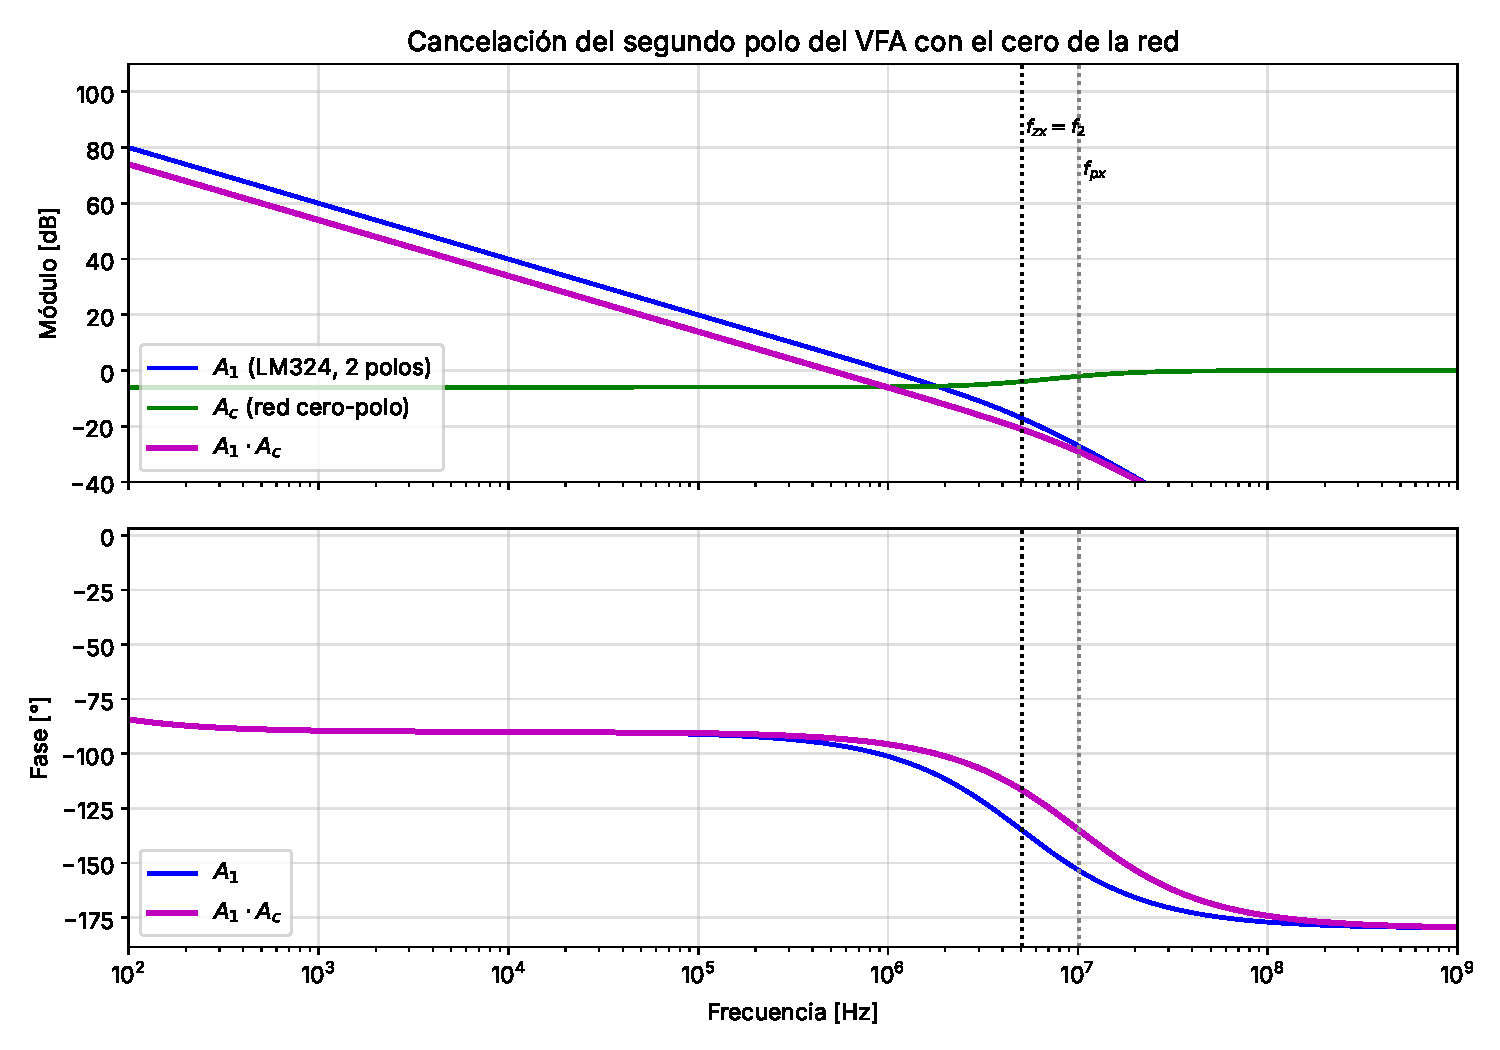
\includegraphics[width=0.85\linewidth,height=0.28\textheight,keepaspectratio]{Imagenes/c3_cancelacion_polo.pdf}
    \caption{Cancelación del segundo polo del VFA con el cero de la red: módulo y fase de $A_1$, $A_c$ y $A_1A_c$.}
    \label{fig:cancelacion_c3}
\end{figure}

\begin{figure}[H]
    \centering
    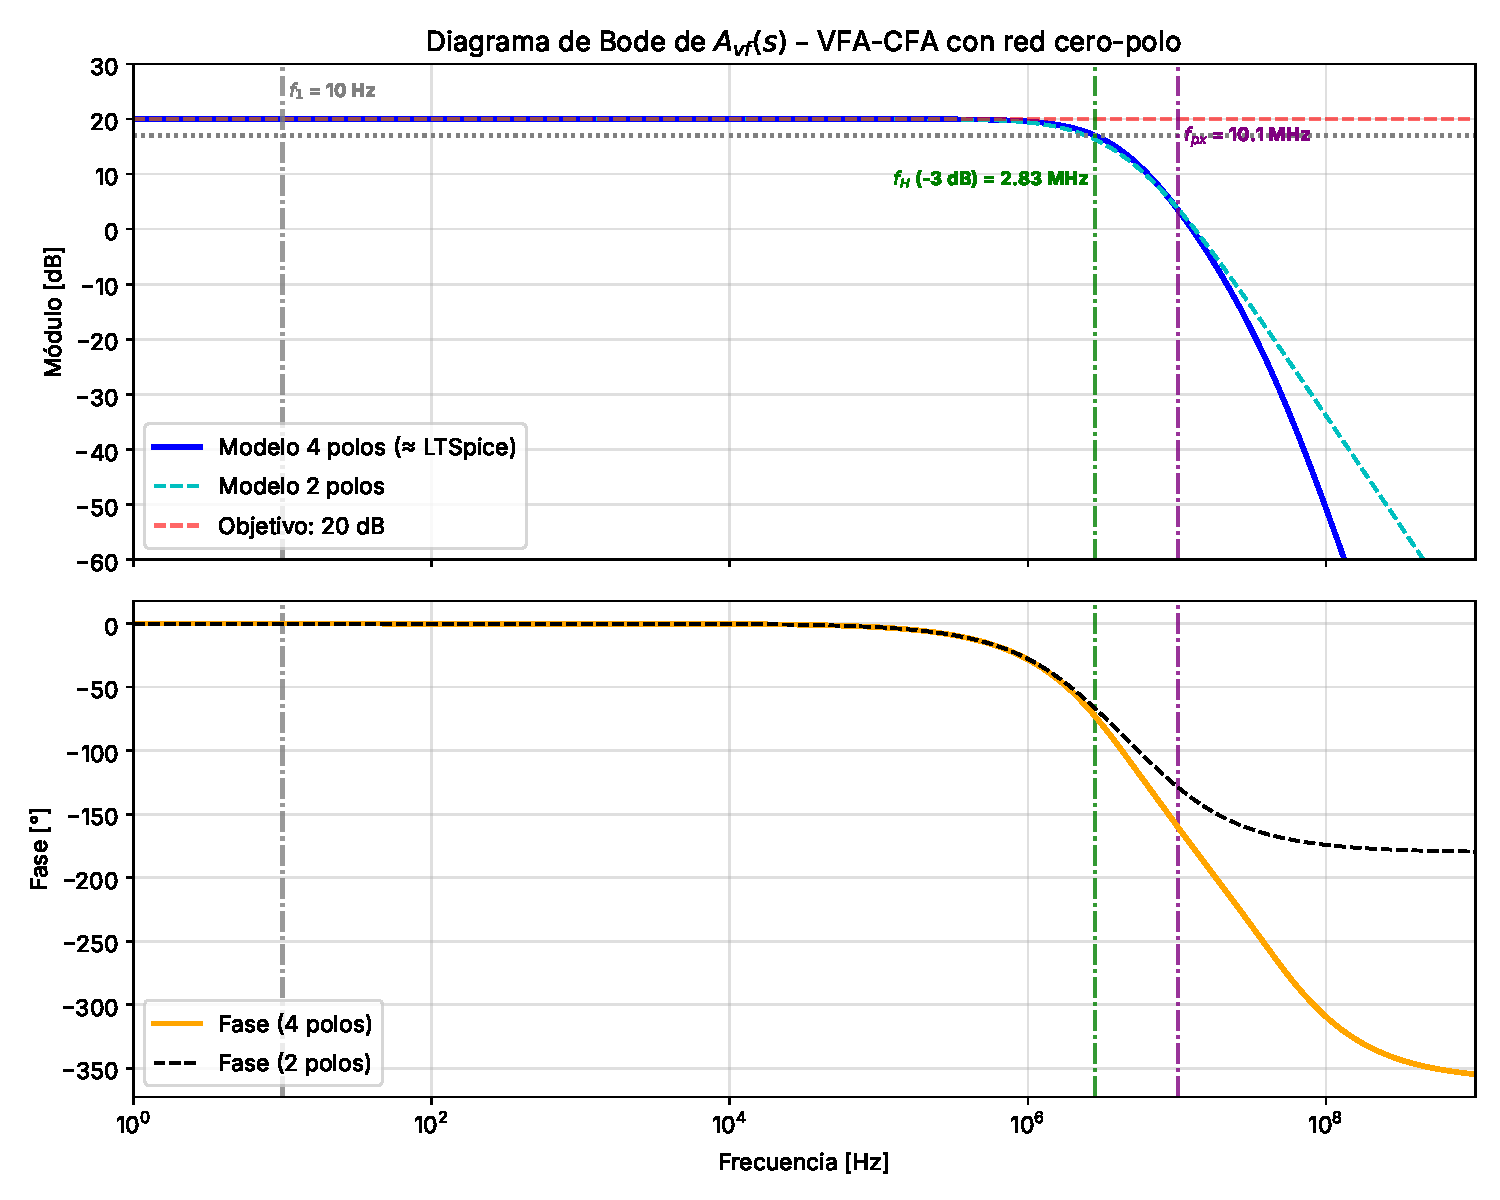
\includegraphics[width=0.85\linewidth,height=0.28\textheight,keepaspectratio]{Imagenes/c3_bode_lazo_cerrado.pdf}
    \caption{Diagrama de Bode a lazo cerrado (modelos de 2 y 4 polos), Caso 3.}
    \label{fig:bode_lc_c3}
\end{figure}

\begin{figure}[H]
    \centering
    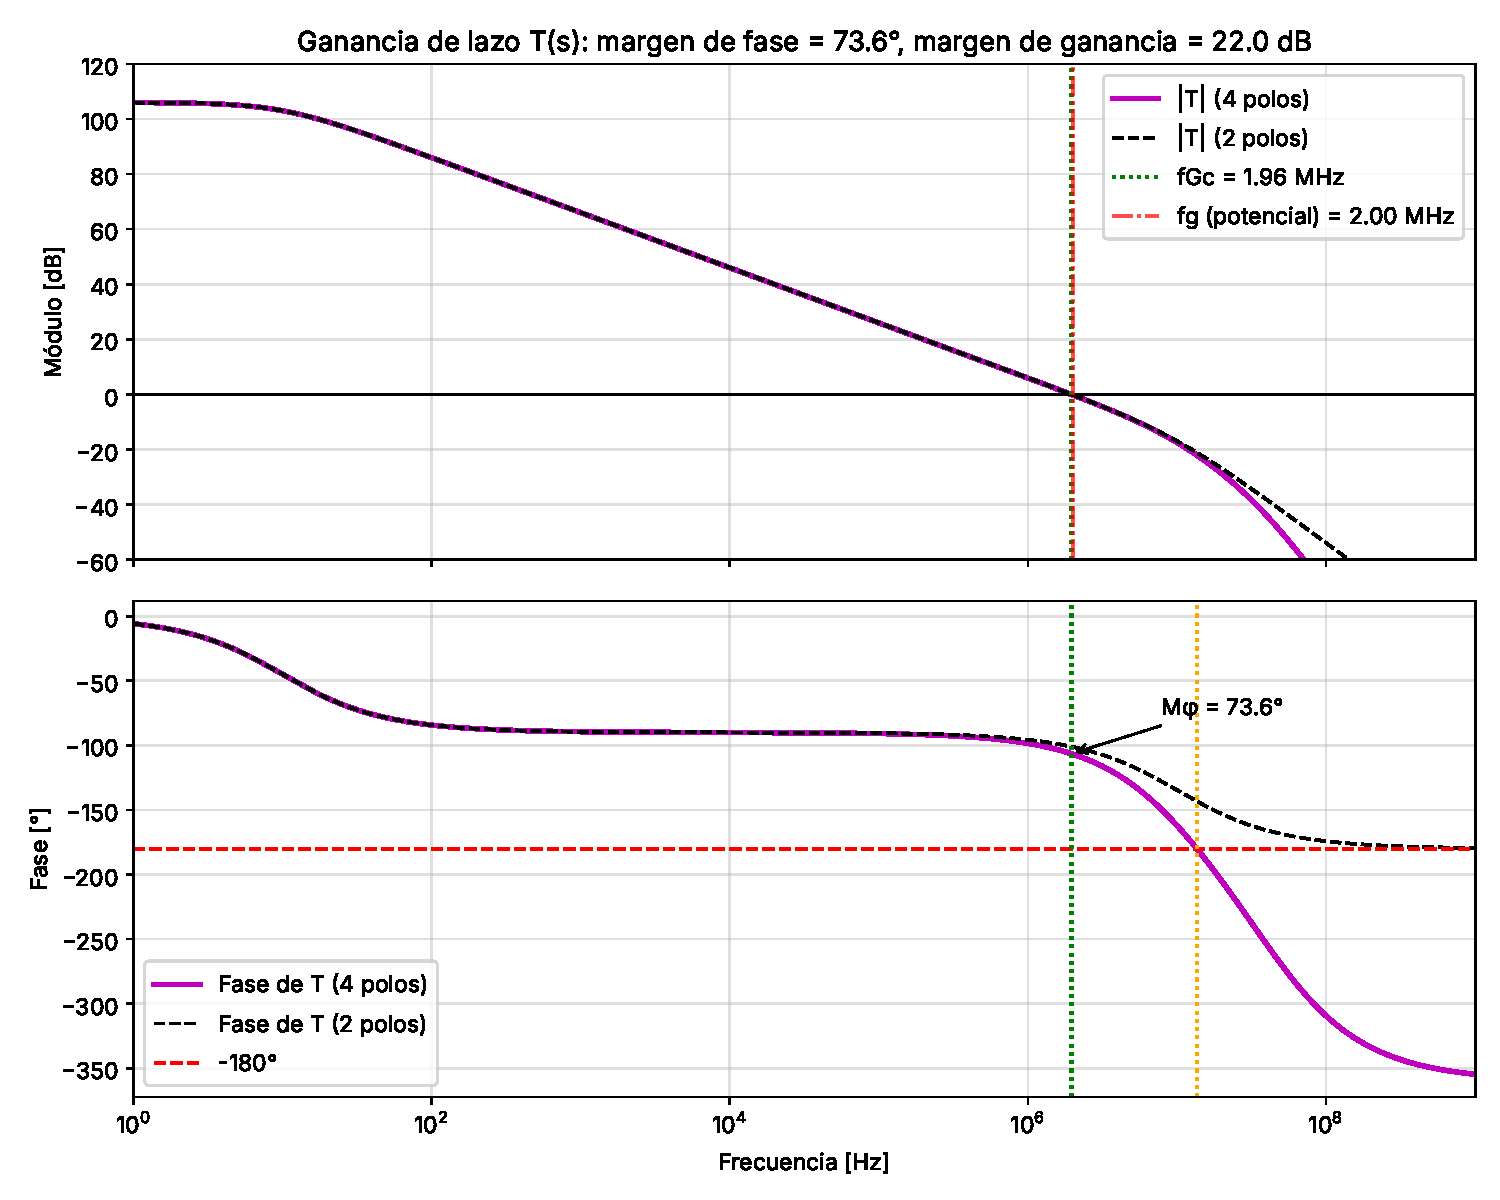
\includegraphics[width=0.85\linewidth,height=0.28\textheight,keepaspectratio]{Imagenes/c3_bode_ganancia_lazo.pdf}
    \caption{Diagrama de Bode de la ganancia de lazo, Caso 3: frecuencia crítica y margen de fase.}
    \label{fig:bode_lazo_c3}
\end{figure}

\paragraph{Comparación con el Caso 2.} La \autoref{tab:comp_teo_c3} y la \autoref{fig:comparacion_c3} muestran la mejora: con el mismo $T_0$ y $f_g$, el margen de fase sube $\ang{7,8}$ y el sobrepico desaparece, a costa de un ancho de banda real $\approx7\,\mathrm{\char37}$ menor (respuesta más amortiguada).

\begin{table}[H]
\centering
\caption{Caso 2 contra Caso 3 (teoría, modelo de 4 polos).}
\label{tab:comp_teo_c3}
\begin{tabular}{lcc}
\toprule
\textbf{Magnitud} & \textbf{Caso 2 (sin red)} & \textbf{Caso 3 (con red)} \\
\midrule
Frecuencia crítica $f_{Gc}$ [MHz] & 1,873 & 1,958 \\
Margen de fase [$^\circ$] & 65,74 & 73,58 \\
Margen de ganancia [dB] & 23,2 & 22,0 \\
Ancho de banda real ($-3$ dB) [MHz] & 3,039 & 2,826 \\
Factor de calidad $Q_p$ & 0,681 & 0,503 \\
Sobrepico \%OS (escalón) [\%] & 3,36 & sin sobrepico \\
\bottomrule
\end{tabular}
\end{table}

\begin{figure}[H]
    \centering
    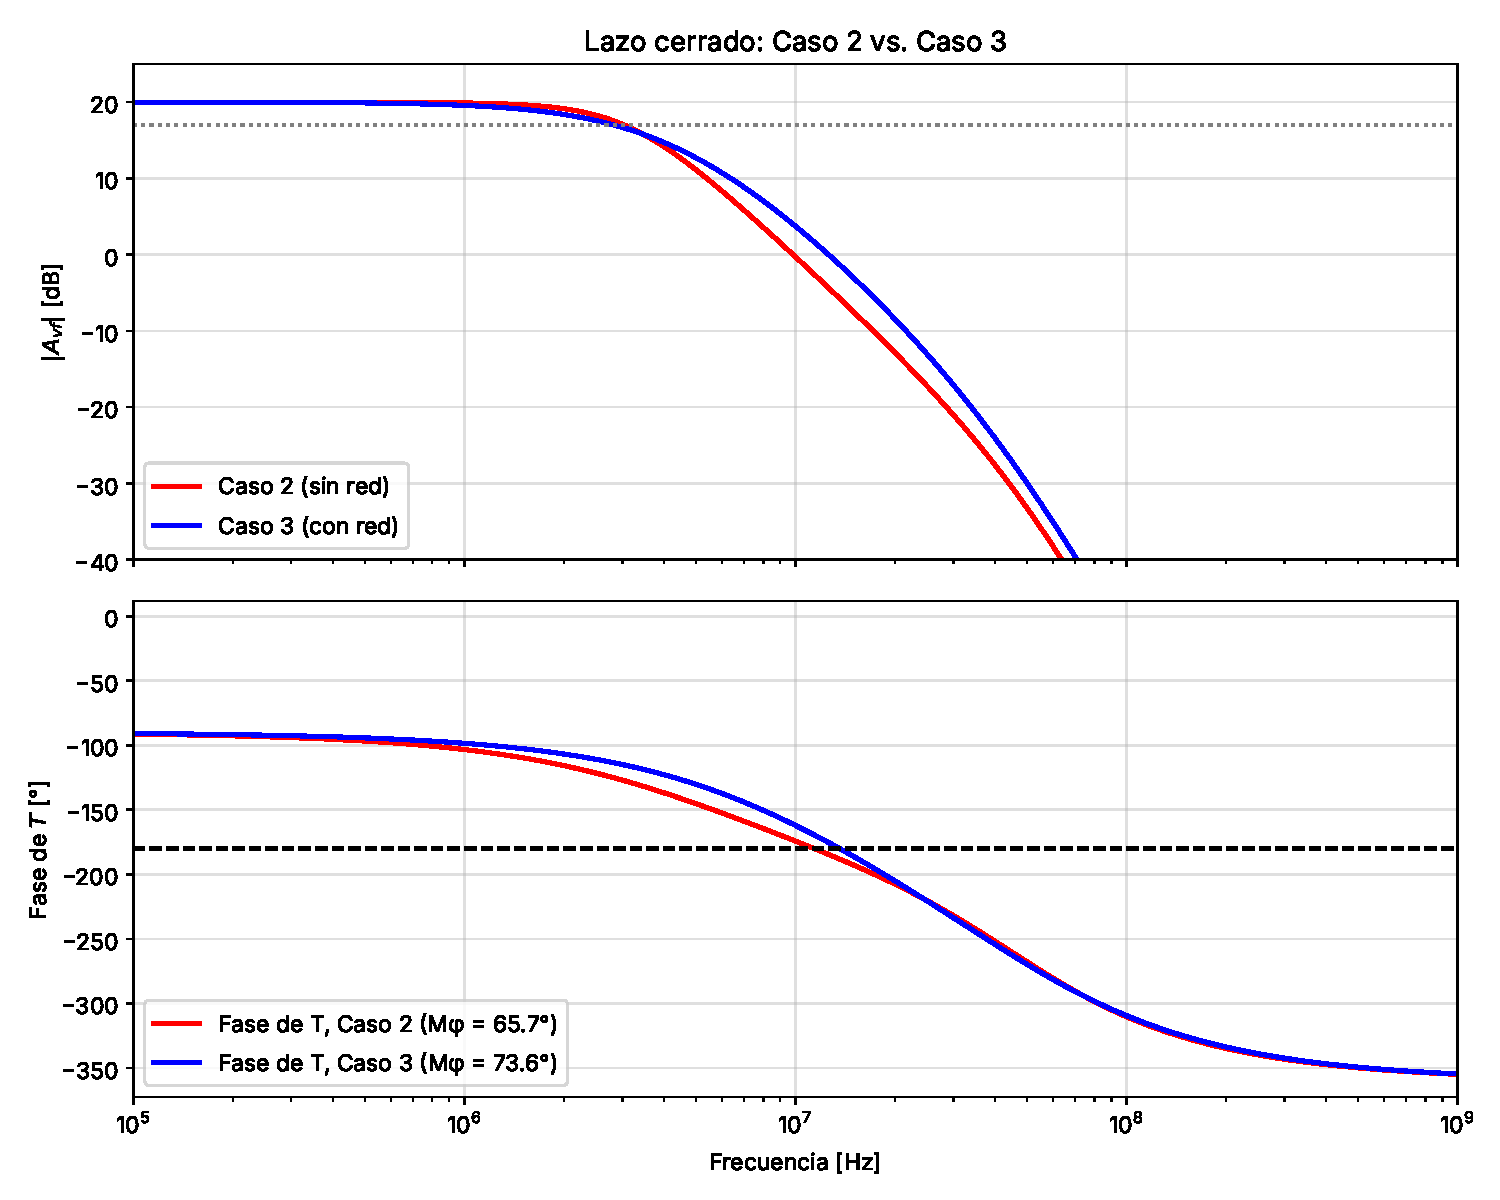
\includegraphics[width=0.85\linewidth,height=0.28\textheight,keepaspectratio]{Imagenes/c3_comparacion_caso2.pdf}
    \caption{Lazo cerrado y fase de $T$: Caso 2 contra Caso 3.}
    \label{fig:comparacion_c3}
\end{figure}

\paragraph{Sensibilidad al valor de $r_i$.} Con $r_i$ entre $0$ y $\SI{50}{\ohm}$ el margen de fase del modelo de cuatro polos varía entre $\ang{76,2}$ y $\ang{69,7}$ (\autoref{tab:ri_c3}); en todos los casos supera al del Caso 2 con el mismo $r_i$.

\begin{table}[H]
\centering
\caption{Sensibilidad al valor de $r_i$ (modelo de 4 polos), Caso 3.}
\label{tab:ri_c3}
\begin{tabular}{cccccc}
\toprule
$r_i$ [$\Omega$] & $R_{eff}'$ [$\Omega$] & $f_{Gc}$ [MHz] & $M_\varphi$ [$^\circ$] & $M_G$ [dB] & BW [MHz] \\
\midrule
0 & 820 & 1,963 & 76,2 & 26,3 & 2,637 \\
10 & 1220 & 1,961 & 74,9 & 23,7 & 2,731 \\
20 & 1620 & 1,958 & 73,6 & 22,0 & 2,826 \\
30 & 2020 & 1,954 & 72,3 & 20,9 & 2,920 \\
50 & 2820 & 1,943 & 69,7 & 19,3 & 3,093 \\
\bottomrule
\end{tabular}
\end{table}

\paragraph{Respuesta al escalón teórica.} La \autoref{fig:escalon_teorico_c3} muestra la respuesta a un escalón de $\SI{0,1}{V}$ (salida de $\SI{1}{V}$) del Caso 3 y la \autoref{fig:escalon_comparacion_c3} la compara con la del Caso 2. En el Caso 3 no hay sobrepico ($\mathrm{\char37}OS<0{,}05\,\mathrm{\char37}$), por lo que la fórmula de la \autoref{eq:zeta} no es aplicable: la ausencia de sobrepico indica $\zeta \gtrsim 0{,}9$, es decir $M_\varphi \gtrsim 73^\circ$ por la \autoref{eq:MF_exacta}, y la mejora se constata comparando con el sobrepico del Caso 2 ($3{,}36\,\mathrm{\char37}$).

\begin{figure}[H]
    \centering
    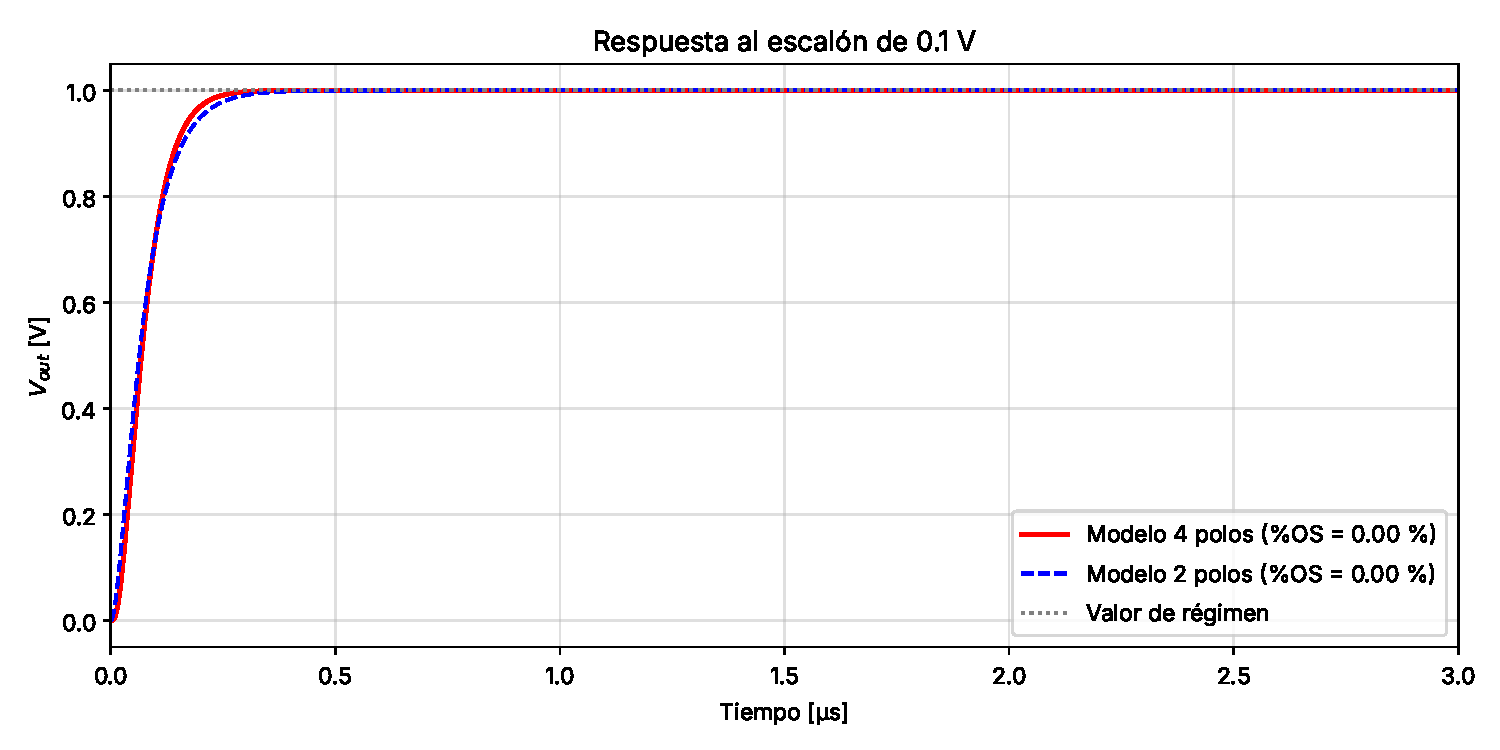
\includegraphics[width=0.85\linewidth,height=0.28\textheight,keepaspectratio]{Imagenes/c3_escalon_teorico.pdf}
    \caption{Respuesta al escalón teórica (2 y 4 polos), Caso 3.}
    \label{fig:escalon_teorico_c3}
\end{figure}

\begin{figure}[H]
    \centering
    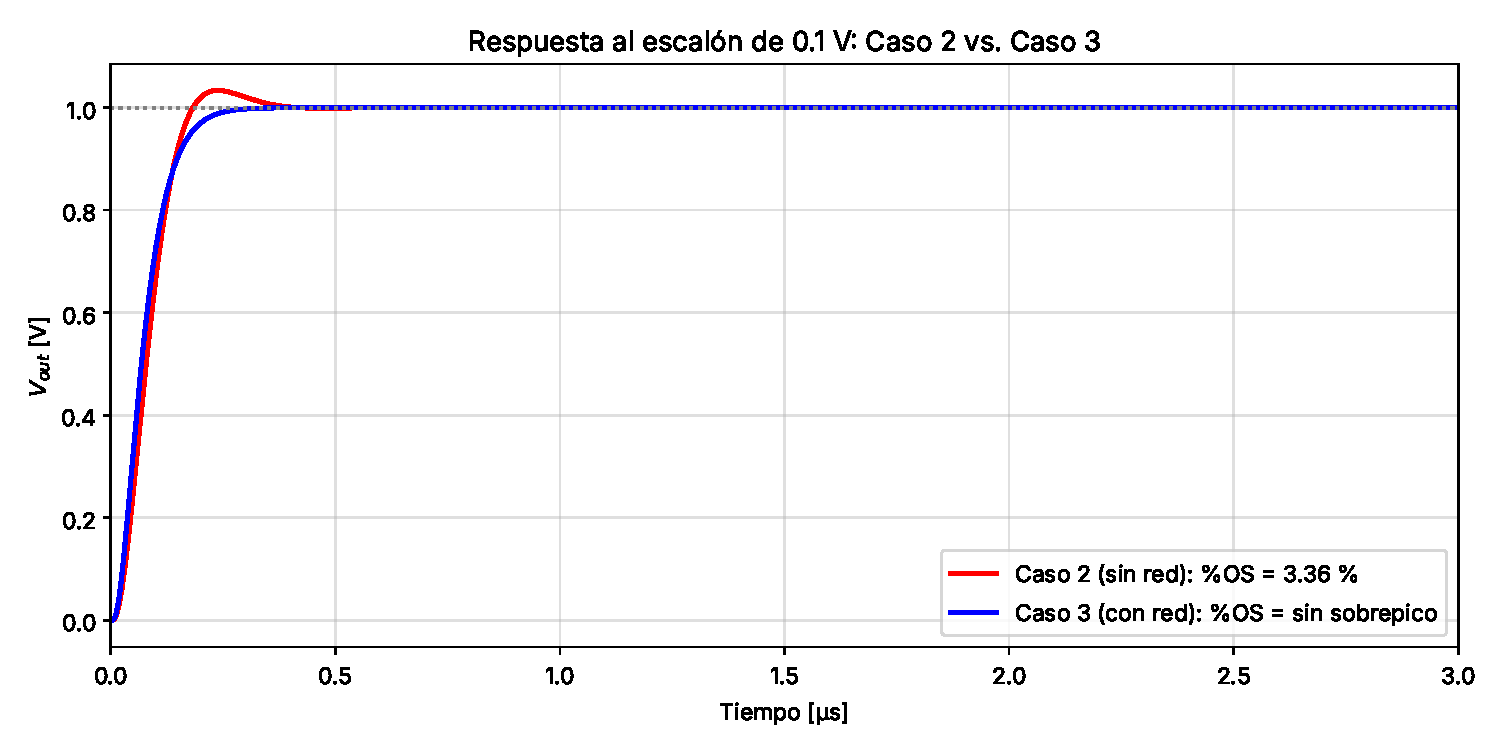
\includegraphics[width=0.85\linewidth,height=0.28\textheight,keepaspectratio]{Imagenes/c3_escalon_comparacion.pdf}
    \caption{Respuesta al escalón teórica: Caso 2 contra Caso 3.}
    \label{fig:escalon_comparacion_c3}
\end{figure}

\subsection{Simulación}
\label{sec:simulacion_c3}

Se simularon en LTSpice los mismos tres circuitos del Caso 2 (\autoref{fig:circuito_VFA_CFA_red}), agregando la red $R_x\parallel C_x$, $R_y$ entre la salida del LM324 y la entrada no inversora del LM6181, con $R_x=R_y=\SI{1}{k\ohm}$, $C_x=\SI{31,45}{pF}$ y $R_1'=\SI{21,03}{\ohm}$ ($R_2=\SI{820}{\ohm}$, $R_i=\SI{1}{k\ohm}$, $R_f=\SI{9}{k\ohm}$).

\begin{figure}[H]
    \centering
    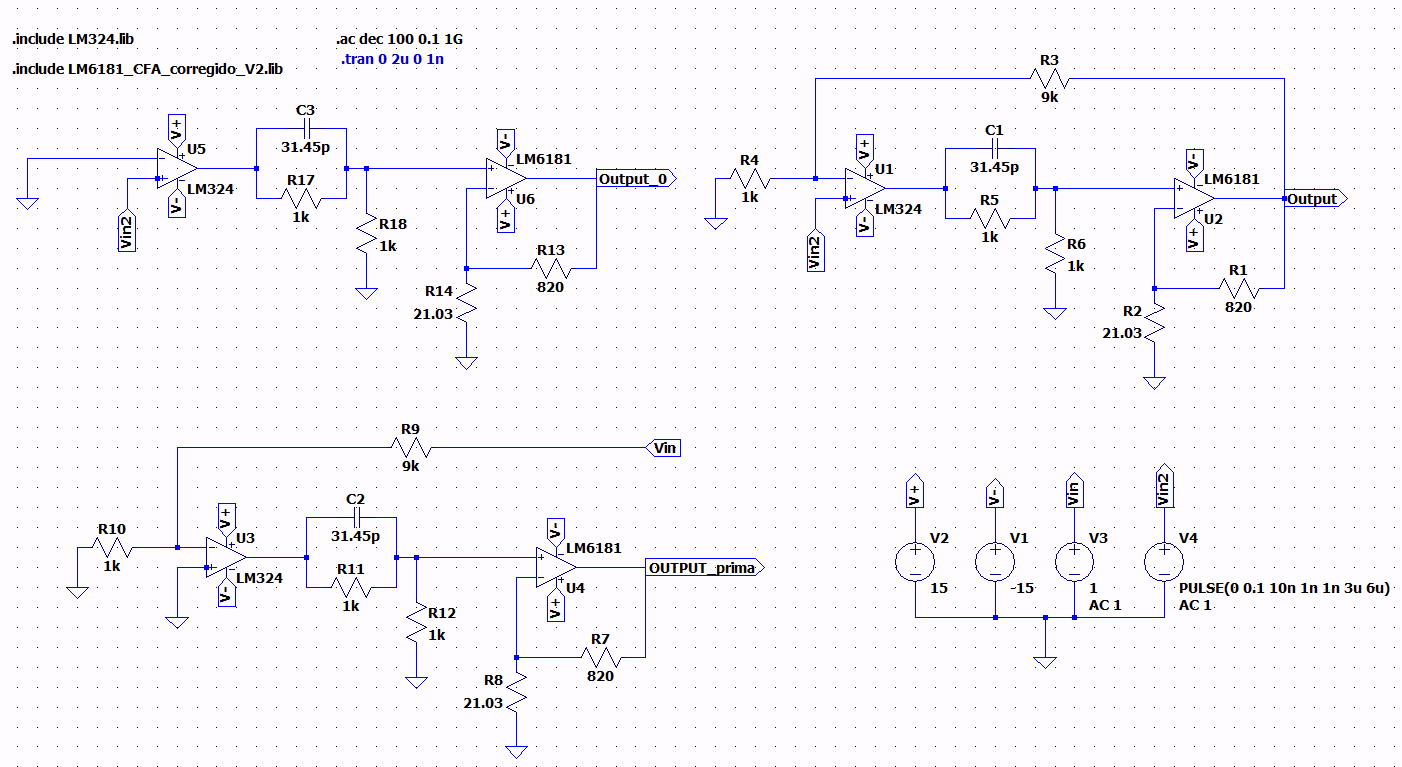
\includegraphics[width=1.0\linewidth,height=0.28\textheight,keepaspectratio]{Imagenes/c3_sim_circuitos.png}
    \caption{Esquemático VFA-CFA con red cero-polo en LTSpice: lazo abierto (arriba a la izquierda), lazo cerrado (arriba a la derecha) y ganancia de lazo (abajo).}
    \label{fig:circuito_VFA_CFA_red}
\end{figure}

\subsubsection{Respuesta en frecuencia a lazo abierto}
La \autoref{fig:rta_frec_open_loop_c3} muestra una ganancia en banda media de $A_{d0}A_c(0)G_0' = 100\text{ dB} + 26\text{ dB} = 126\text{ dB}$ (igual que el Caso 2), con el polo dominante en $f_1=\SI{10}{Hz}$. La fase se mantiene cerca de $-90^\circ$ hasta varios MHz: la red cancela el cambio de pendiente que el segundo polo del VFA produciría en $f_2=\SI{5,06}{MHz}$, y el atraso de fase aparece recién con el polo de la red y los del CFA.

\begin{figure}[H]
    \centering
    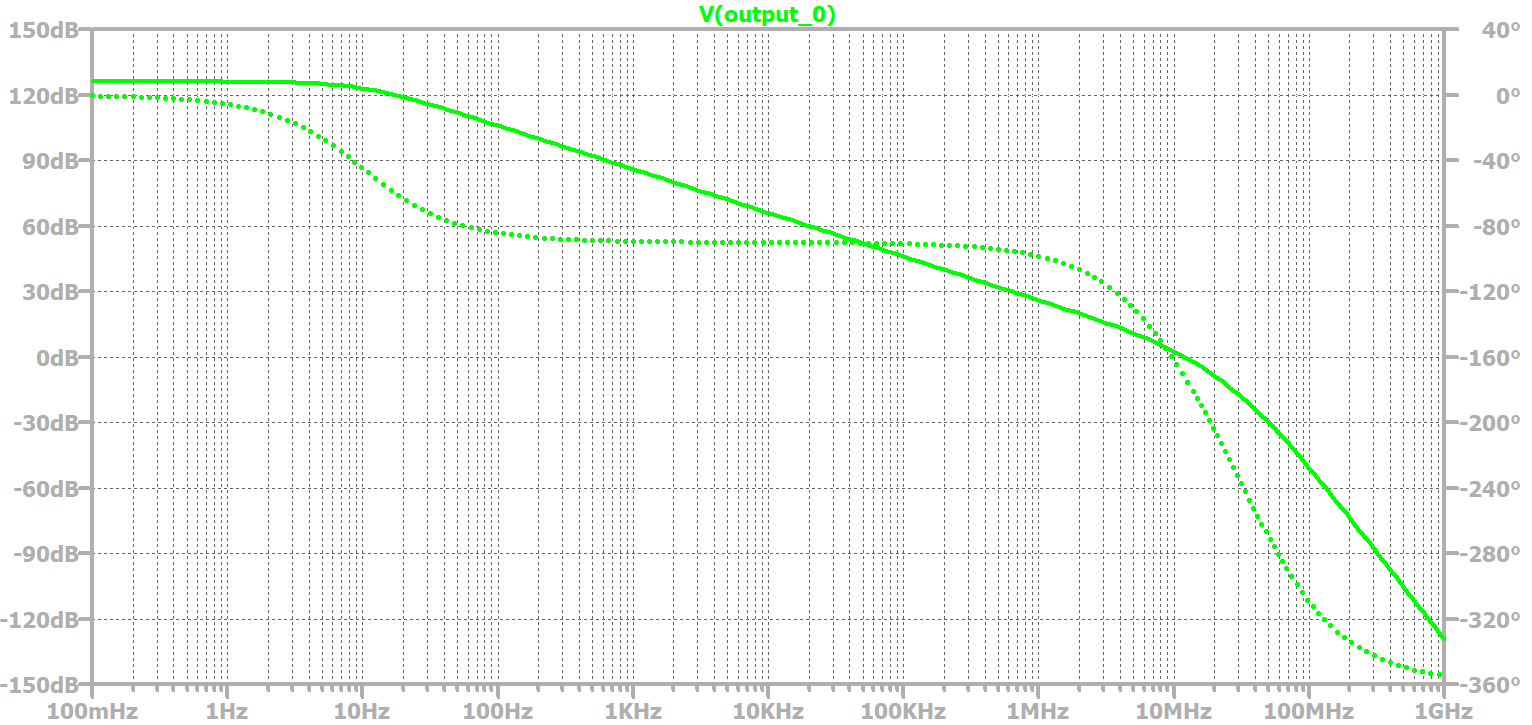
\includegraphics[width=0.85\linewidth,height=0.28\textheight,keepaspectratio]{Imagenes/c3_sim_lazo_abierto.png}
    \caption{Respuesta en frecuencia a \textbf{lazo abierto} del compuesto con red cero-polo (módulo y fase).}
    \label{fig:rta_frec_open_loop_c3}
\end{figure}

\subsubsection{Respuesta en frecuencia de la ganancia de lazo}
En la \autoref{fig:rta_frec_loop_c3} se midió sobre la curva de $-T$ (\texttt{V(output\_prima)}) el cruce por \SI{0}{dB} en $f_{Gc} = \SI{1,957}{MHz}$, donde la fase es $M_\varphi = \ang{73,62}$ (el modelo de cuatro polos predice \SI{1,958}{MHz} y \ang{73,58}). La ganancia de lazo en continua es de \SI{106}{dB}, igual que en el Caso 2.

\begin{figure}[H]
    \centering
    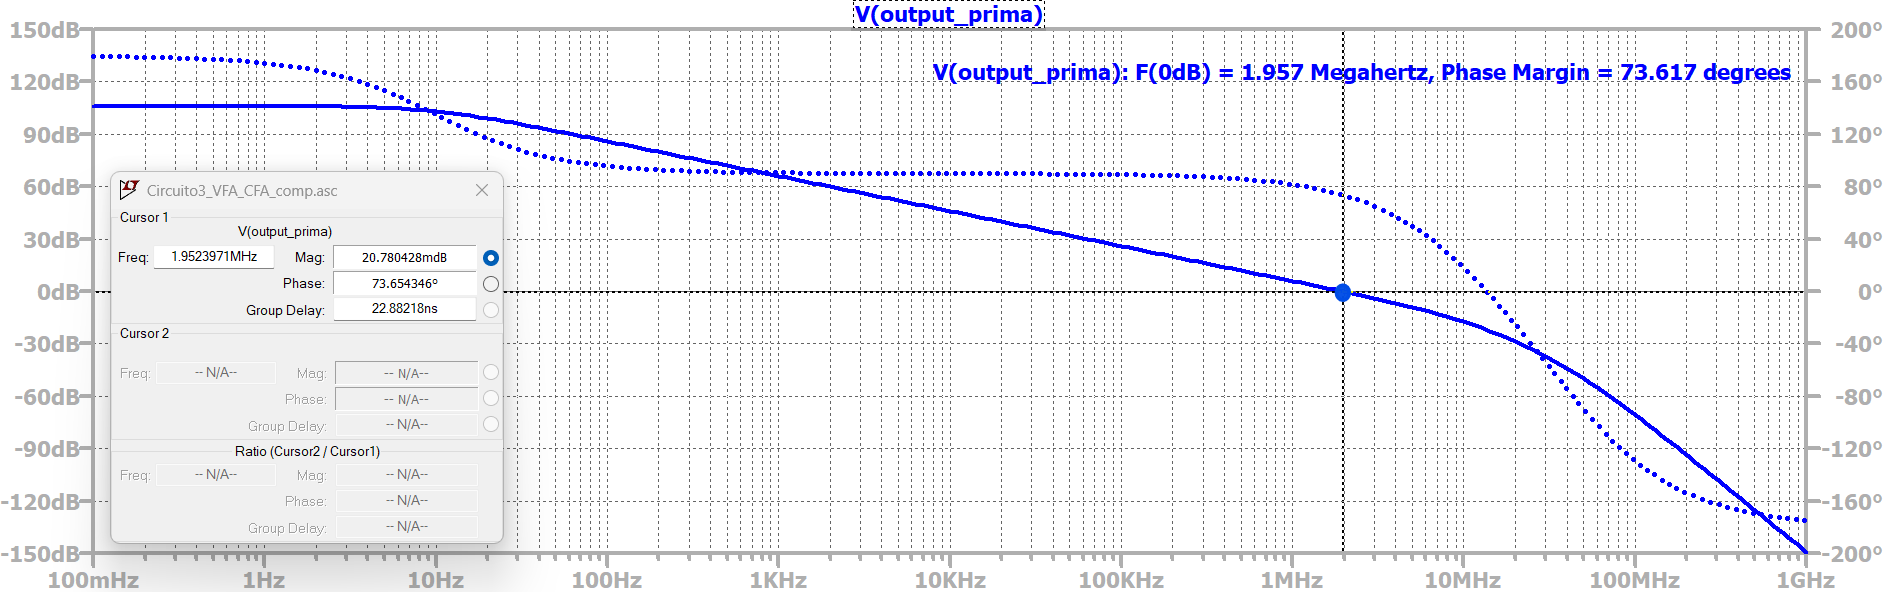
\includegraphics[width=0.85\linewidth,height=0.28\textheight,keepaspectratio]{Imagenes/c3_sim_lazo_T.png}
    \caption{Respuesta en frecuencia de la \textbf{ganancia de lazo} ($-T$): $f_{Gc} = \SI{1,957}{MHz}$ y $M_\varphi = \ang{73,62}$.}
    \label{fig:rta_frec_loop_c3}
\end{figure}

\subsubsection{Respuesta en frecuencia a lazo cerrado}
La \autoref{fig:rta_frec_close_loop_c3} confirma la ganancia en banda media de $\SI{20}{dB}$ ($\SI{19,99996}{dB}$ a $\SI{30}{Hz}$), sin sobrepico. Con el cursor a $\SI{17}{dB}$ se obtuvo $\SI{17,004}{dB}$ a $\SI{2,815}{MHz}$ ($-3{,}00$ dB respecto de banda media); interpolando al punto de $-3{,}01$ dB resulta un ancho de banda real $f_H \approx \SI{2,82}{MHz}$ (el modelo de cuatro polos predice $\SI{2,826}{MHz}$).

\begin{figure}[H]
    \centering
    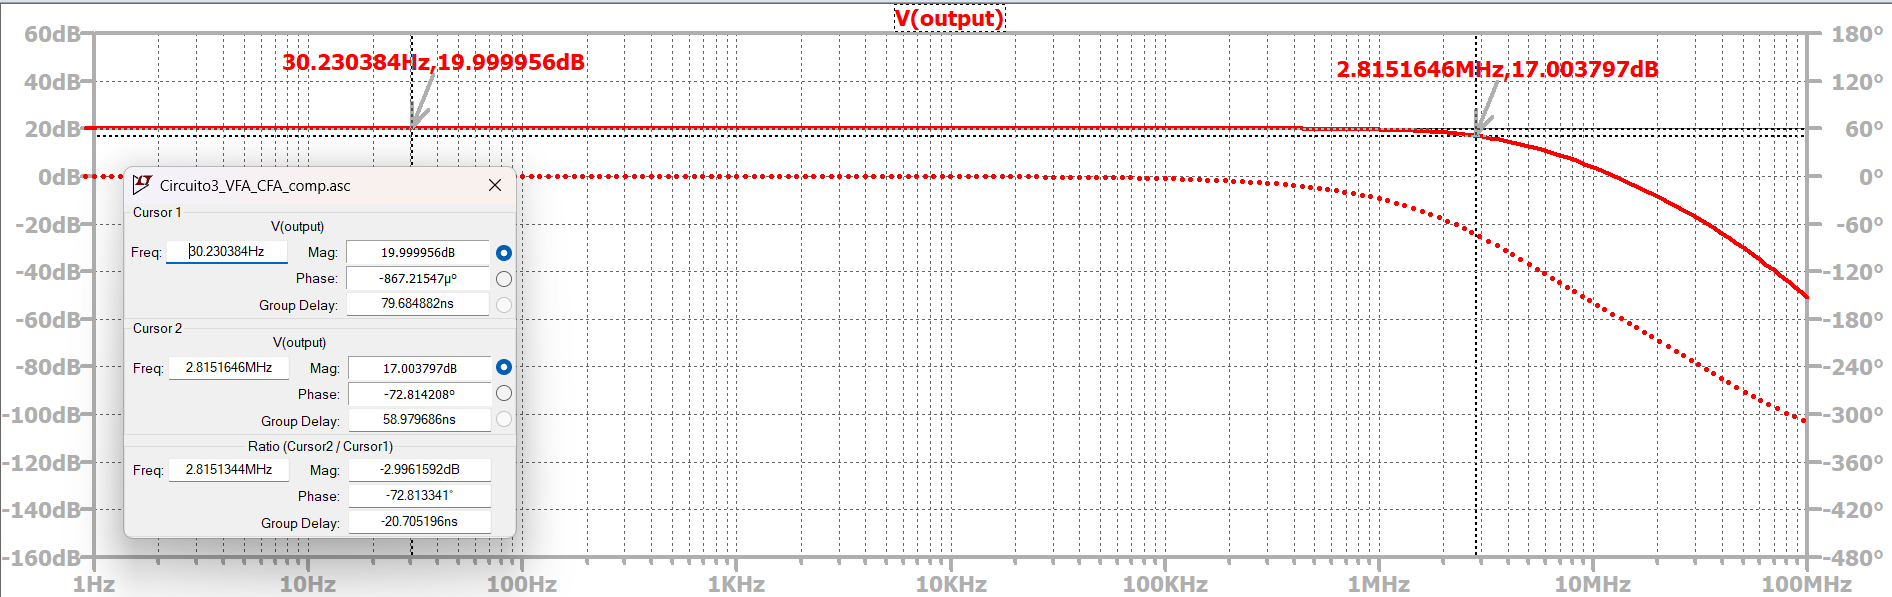
\includegraphics[width=0.85\linewidth,height=0.28\textheight,keepaspectratio]{Imagenes/c3_sim_lazo_cerrado.png}
    \caption{Respuesta en frecuencia a \textbf{lazo cerrado}.}
    \label{fig:rta_frec_close_loop_c3}
\end{figure}

\subsubsection{Respuesta al escalón}
Se aplicó un escalón de $\SI{0,1}{V}$ (salida de $\SI{1}{V}$) con flancos de $\SI{1}{ns}$. La salida (\autoref{fig:rta_step_c3}) crece de forma monótona hasta $\SI{1}{V}$ y se asienta en $\approx\SI{300}{ns}$, \emph{sin sobrepico visible}, como predice el modelo. El Caso 2, con el mismo escalón, tenía un sobrepico de $3{,}35\,\mathrm{\char37}$ (\autoref{fig:rta_step_c2}). Como no hay sobrepico no puede estimarse $\zeta$ ni el margen de fase con las \autoref{eq:zeta} y \autoref{eq:MF_exacta}; solo se concluye que $\zeta \gtrsim 0{,}9$ y $M_\varphi \gtrsim 73^\circ$, consistente con los $\ang{73,6}$ medidos en el lazo.

\begin{figure}[H]
    \centering
    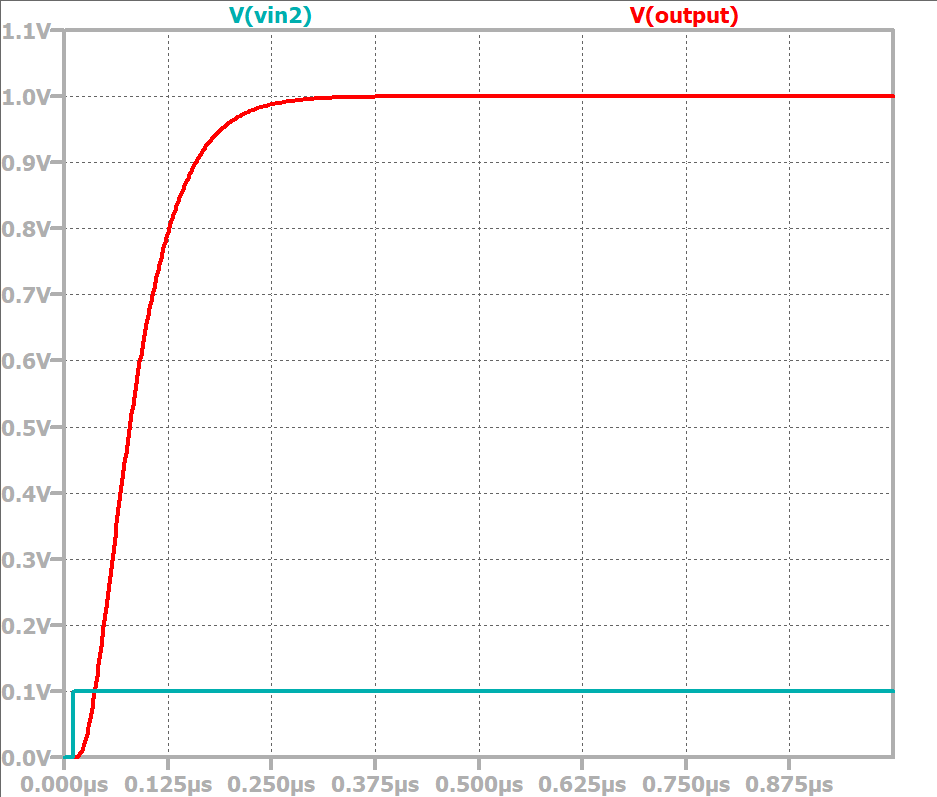
\includegraphics[width=0.85\linewidth,height=0.28\textheight,keepaspectratio]{Imagenes/c3_sim_escalon.png}
    \caption{Respuesta al escalón de $\SI{0,1}{V}$ (LTSpice), Caso 3: sin sobrepico.}
    \label{fig:rta_step_c3}
\end{figure}

\subsection{Comparación de resultados}
\label{sec:comparacion_c3}

La \autoref{tab:final_c3} compara los valores analíticos (dos polos), el modelo de cuatro polos y las mediciones de LTSpice, y la \autoref{tab:comp_sim_c3} contrasta los dos compuestos con medidas de simulación.

\begin{table}[H]
\centering
\caption{Comparación entre teoría y simulación (VFA-CFA con red). Error $= (\text{teórico}-\text{LTSpice})/\text{LTSpice}$.}
\label{tab:final_c3}
\small
\setlength{\tabcolsep}{4pt}
\setlength{\tabcolsep}{4pt}
\begin{tabularx}{\textwidth}{>{\raggedright\arraybackslash}X c c c c c}
\toprule
\textbf{Magnitud} & \textbf{Analítico} & \textbf{4 polos} & \textbf{LTSpice} & \textbf{Err. anal. [\%]} & \textbf{Err. 4p [\%]} \\
\midrule
Ancho de banda potencial $f_g$ [MHz] & 2,000 & -- & -- & -- & -- \\
Cruce de $T$ exacto $f_{Gc}$ [MHz] & 1,963 & 1,958 & 1,957 & $+0{,}3$ & $0{,}0$ \\
Margen de fase del lazo [$^\circ$] & 79,02 & 73,58 & 73,62 & $+7{,}3$ & $0{,}0$ \\
Frecuencia de polos $f_p$ [MHz] & 4,499 & 4,391 & -- & -- & -- \\
Ancho de banda real $f_H$ [MHz] & 2,455 & 2,826 & 2,82 & $-13{,}0$ & $+0{,}1$ \\
Sobrepico \%OS [\%] & 0 & 0 & sin sobrepico & -- & -- \\
\bottomrule
\end{tabularx}
\end{table}

\begin{table}[H]
\centering
\caption{Caso 2 contra Caso 3: modelo de 4 polos y simulación en LTSpice.}
\label{tab:comp_sim_c3}
\small
\setlength{\tabcolsep}{4pt}
\begin{tabular}{lcccc}
\toprule
 & \multicolumn{2}{c}{\textbf{Caso 2 (sin red)}} & \multicolumn{2}{c}{\textbf{Caso 3 (con red)}} \\
\textbf{Magnitud} & 4 polos & LTSpice & 4 polos & LTSpice \\
\midrule
Frecuencia crítica $f_{Gc}$ [MHz] & 1,873 & 1,873 & 1,958 & 1,957 \\
Margen de fase del lazo [$^\circ$] & 65,74 & 65,78 & 73,58 & 73,62 \\
Ancho de banda real [MHz] & 3,039 & 3,04 & 2,826 & 2,82 \\
Sobrepico \%OS [\%] & 3,36 & 3,35 & 0 & sin sobrepico \\
\bottomrule
\end{tabular}
\end{table}

\subsection{Análisis y conclusión parcial}
\label{sec:concl_c3}

\begin{itemize}
    \item La red cero-polo cancela el segundo polo del LM324 y desplaza el nuevo segundo polo de $\SI{5,06}{MHz}$ a $\SI{10,12}{MHz}$. Con $T_0$ y $f_g$ iguales a los del Caso 2, el margen de fase medido mejora de $\ang{65,78}$ a $\ang{73,62}$ (mejora de $\ang{7,8}$, igual a la prevista por el modelo) y el sobrepico del escalón pasa de $3{,}35\,\mathrm{\char37}$ a nulo.
    \item La simulación coincide con el modelo de cuatro polos con errores menores al $0{,}3\,\mathrm{\char37}$ en $f_{Gc}$, margen de fase y ancho de banda, lo que valida el modelo del compuesto con la red. El modelo de dos polos sobreestima el margen de fase en $\approx5^\circ$ ($79{,}0^\circ$ contra $73{,}6^\circ$), porque desprecia el atraso de fase de los polos del CFA, y subestima el ancho de banda ($13\,\mathrm{\char37}$).
    \item La mejora tiene un costo: la respuesta queda más amortiguada y el ancho de banda real baja de $\SI{3,04}{MHz}$ a $\SI{2,82}{MHz}$ ($\approx7\,\mathrm{\char37}$), y se necesita duplicar la ganancia del CFA, lo que aumenta $R_{eff}'$ y baja su polo de $\SI{27,2}{MHz}$ a $\SI{20,5}{MHz}$ (sigue siendo $10$ veces $f_g$). Aun así el ancho de banda es unas $8$ veces el del compuesto VFA-VFA del Caso 1 ($\SI{345}{kHz}$).
    \item Como no hay sobrepico en el escalón, el margen de fase no puede estimarse por ese método; solo se acota ($M_\varphi \gtrsim 73^\circ$), consistente con el valor medido en el lazo.
    \item La cancelación es exacta solo en el modelo: en el circuito real depende de las tolerancias de $R_x$ y $C_x$ y de la impedancia de salida del VFA, por lo que el cero puede correrse y la mejora real ser menor.
\end{itemize}
